%%%%%%%%%%%%%%%%%%%%%%%%%%%%%%%%%%%%%%%%%
% University/School Laboratory Report
% LaTeX Template
% Version 3.1 (25/3/14)
%
% This template has been downloaded from:
% http://www.LaTeXTemplates.com
%
% Original author:
% Linux and Unix Users Group at Virginia Tech Wiki 
% (https://vtluug.org/wiki/Example_LaTeX_chem_lab_report)
%
% License:
% CC BY-NC-SA 3.0 (http://creativecommons.org/licenses/by-nc-sa/3.0/)
%
%%%%%%%%%%%%%%%%%%%%%%%%%%%%%%%%%%%%%%%%%

%----------------------------------------------------------------------------------------
%	PACKAGES AND DOCUMENT CONFIGURATIONS
%----------------------------------------------------------------------------------------

\documentclass{article}
\usepackage[left=2cm,right=2cm,top=2cm,bottom=2cm]{geometry}
\usepackage[utf8]{vietnam}
\usepackage[version=3]{mhchem} % Package for chemical equation typesetting
\usepackage{siunitx} % Provides the \SI{}{} and \si{} command for typesetting SI units
\usepackage{graphicx} % Required for the inclusion of images
\usepackage{natbib} % Required to change bibliography style to APA
\usepackage{amsmath} % Required for some math elements 
\usepackage{wrapfig}
\usepackage{subcaption}

\usepackage{listings}
\renewcommand{\lstlistingname}{Mã nguồn}
\usepackage{xcolor}

\definecolor{codegreen}{rgb}{0,0.6,0}
\definecolor{codegray}{rgb}{0.5,0.5,0.5}
\definecolor{codepurple}{rgb}{0.58,0,0.82}
\definecolor{backcolour}{rgb}{0.95,0.95,0.92}

\lstdefinestyle{mystyle}{
    backgroundcolor=\color{backcolour},   
    commentstyle=\color{codegreen},
    keywordstyle=\color{magenta},
    numberstyle=\tiny\color{codegray},
    stringstyle=\color{codepurple},
    basicstyle=\ttfamily\footnotesize,
    breakatwhitespace=false,         
    breaklines=true,                 
    captionpos=b,                    
    keepspaces=true,                 
    numbers=left,                    
    numbersep=5pt,                  
    showspaces=false,                
    showstringspaces=false,
    showtabs=false,                  
    tabsize=2
}


\lstset{style=mystyle}


%\setlength\parindent{1pt} % Removes all indentation from paragraphs

\renewcommand{\labelenumi}{\alph{enumi}.} % Make numbering in the enumerate environment by letter rather than number (e.g. section 6)

% Keywords command
\providecommand{\keywords}[1]
{
  \small	
  \textbf{\textit{Từ khóa:}} #1
}

%\usepackage{times} % Uncomment to use the Times New Roman font

%----------------------------------------------------------------------------------------
%	DOCUMENT INFORMATION
%----------------------------------------------------------------------------------------

\title{HỆ KHUYẾN NGHỊ CỘNG TÁC \\ ĐỒNG TÁC GIẢ} % Title

\author{Nhóm: \textsc{Project III}} % Author name

\date{\today} % Date for the report

%\setlength{\parindent}{4em}

\begin{document}

\maketitle % Insert the title, author and date

\begin{center}
\begin{tabular}{l r}
% Date Performed: & January 1, 2020 \\ % Date the experiment was performed
Thành Viên: & Lê Văn Linh \\ % Partner names
& Trần Tùng Lâm  \\
& Nguyễn Sỹ Đức \\
& Bùi Quang Đức \\
Giảng Viên: & Trần Đình Khang % Instructor/supervisor
\end{tabular}
\end{center}

% If you wish to include an abstract, uncomment the lines below
\begin{abstract}
Mạng đồng tác giả là mạng lưới học thuật giữa các nhà nghiên cứu viết chung bài
báo khoa học và mức độ kết hợp đồng tác giả có thể được đặc trưng bởi các độ đo liên kết.
Dựa trên các đặc trưng đó, có thể xây dựng nhiều bài toán có ý nghĩa, trong đó có khuyến
nghị cộng tác, gợi ý các tác giả có thể kết hợp trong tương lai hoặc tăng cường hợp tác. Bài
báo này đề xuất một số độ đo liên kết mới dựa trên cộng đồng tác giả, kịch bản thiết lập
bảng ứng viên động theo thời gian và xây dựng hệ khuyến nghị đồng tác giả sử dụng các độ
đo đó.
\end{abstract}

\hspace{10pt}
\keywords{mạng đồng tác giả, độ đo liên kết, khuyến nghị cộng tác}

%----------------------------------------------------------------------------------------
%	SECTION 1
%----------------------------------------------------------------------------------------

\section{Sơ lược đề tài}

\subsection{Mục đích bài toán}

\indent Trong nghiên cứu khoa học, một bài báo thường là sản phẩm của một nhóm tác giả. Việc thể hiện mối liên quan giữa các tác giả với nhau dựa trên các tiêu chí như chủ đề nghiên cứu, số lượng bài báo nghiên cứu chung,... là một vấn đề đang được quan tâm. Quan hệ ấy có thể được thể hiện dưới dạng một mạng xã hội, gọi là mạng đồng tác giả, với các đỉnh tượng trưng cho một tác giả, các cạnh thể hiện sự liên hệ giữa hai tác giả. Ngoài mục đích được sử dụng như một cơ sở dữ liệu để thực hiện các truy vấn, mạng đồng tác giả còn có thể được khai thác để cung cấp dữ liệu cho mô hình học máy dự đoán một cặp tác giả có thể cùng viết một bài báo trong tương lai hay không, giúp cho tác giả có thể mở rộng mối quan hệ của mình.

% If you have more than one objective, uncomment the below:
%\begin{description}
%\item[First Objective] \hfill \\
%Objective 1 text
%\item[Second Objective] \hfill \\
%Objective 2 text
%\end{description}

\subsection{Mạng đồng tác giả}

Một mạng đồng tác giả có thể được mô tả bằng hàm $G^T=(V^T, E^T, P^T, T)$ trong đó $T=\{t_1, t_2, ..., t_k\}$ là các tập nhãn thời gian; $V^T=\{v_1, v_2, ...\}$ là các tập đỉnh được tạo trong khoảng thời gian T, mỗi nút đại diện cho một tác giả trong cộng đồng nghiên cứu; $P^T=\{p_1, p_2, ...\}$ là tập các bài báo trong thời gian T; $E^T=\{(v_i, v_j, p_k, t_h)\}$ là tập các liên kết giữa các tác giả, thể hiện trong thời gian T, hai tác giả $(v_i, v_j)$ có viết chung bài báo $p_k$ tại nhãn thời gian $t_h$. \\

Ngoài ra, tập đỉnh $V^T$ còn có thể chứa các thuộc tính của từng nút tương ứng với thông tin cá nhân của từng tác giả như quốc tịch, trường đại học / viện nghiên cứu mà họ công tác, các lĩnh vực chuyên ngành. Các thuộc tính này được ký hiệu bằng tập $A^T=\{a_1, a_2, ... a_N\}$, trong đó $a_i$ là vector đặc trưng chứa thông tin của tác giả / đỉnh $v_i$. Các độ đo sự tương đồng giữa hai tác giả sẽ được xây dựng dựa trên thông tin của các tập $E^T$ và $A^T$. \\

Từ mạng đồng tác giả ở thời điểm hiện tại, có thể tính toán được các cặp tác giả tiềm năng liên kết trong tương lai, hay còn gọi là ứng viên đồng tác giả. Kèm theo đó là các độ đo liên kết của các cặp ứng viên đó tạo nên bảng ứng viên đồng tác giả. Xác định các cặp ứng viên đồng tác giả; (u, v) là một cặp ứng viên nếu:
$\exists p \in P^{T1}, t \in T1: (u, v, p, t) \in E^{T1}$ hoặc $\exists z \in V^{T1}, (p_1, p_2) \in P^{T1}, (t_1, t_2) \in T1: (u, z, p_1, t_1), (u, v, p_2, t_2) \in E^{T1}$ \\

Các độ đo liên kết của các cặp ứng viên được tính trong khoảng thời gian T1. Việc gán nhãn sẽ thực hiện ở thời gian T2 (xảy ra sau T1). Gán nhãn 1 cho cặp (u, v) nếu: $\exists p \in P^{T2}, t \in T2: (u,v, p, t) \in E^{T2}$, ngược lại gán nhãn 0. \\

Cho trước một khoảng thời gian T thì $G^T$ là mạng đồng tác giả tương ứng với lát cắt thời gian đó. Bài toán khuyến nghị cộng tác sẽ sử dụng các thông tin từ $G^T$ để đưa ra các khuyến nghị cho một tác giả $v_i$ lựa chọn các ứng viên phù hợp để cộng tác đồng tác giả ở thời gian tiếp theo hoặc khuyến nghị cho một cặp tác giả $(v_i, v_j)$ tiếp tục tăng cường cộng tác đồng tác giả.

\subsection{Hướng giải quyết}

Đầu tiên, từ cơ sở dữ liệu quan hệ bao gồm các bảng (ví dụ Author, Paper, PaperAuthor, v.v) thể hiện thông tin về bài báo và tác giả, xây dựng bảng đồng tác giả (CoAuthorship) với các trường chính là tác giả 1, tác giả 2. Bổ sung thêm các độ đo liên kết giữa các cặp đồng tác giả, các độ đo liên kết này lượng hóa mức độ liên kết giữa cặp tác giả. \\

Tiếp theo, xây dựng bảng ứng viên đồng tác giả từ bảng đồng tác giả với quy tắc: một cặp tác giả (a,b) được gọi là ứng viên đồng tác giả nếu hai người đã từng cùng viết chung một bài báo, hoặc tồn tại một tác giả khác, c, cùng viết báo với hai người này (a và c đã viết chung, b và c đã viết chung). Tương ứng bổ sung các độ đo liên kết giữa các cặp tác giả vừa tìm được này. Ta được bảng ứng viên đồng tác giả, là tập cha của bảng đồng tác giả. \\

Cuối cùng, để xây dựng dữ liệu cho mô hình học máy, ta có thể chia toàn bộ tập dữ liệu thành hai phần: một phần bao gồm các bài báo được viết trong khoảng thời gian T1 (trước thời điểm T nào đó), số bài báo còn lại được viết trong sau thời điểm T, được xếp vào phần còn lại. Nhãn được gán cho các cặp ứng viên thuộc nhóm T1: nếu hai tác giả (u,v) thực sự hợp tác với nhau trong khoảng thời gian T2 thì nhãn là 1, ngược lại nhãn là 0. Từ đó có thể áp dụng các mô hình học máy, học sâu để học ra bộ trọng số có thể dự đoán sự hợp tác với một cặp tác giả nào đó. 
 
\subsection{Mục tiêu}

Mục tiêu môn học này là sinh viên có thể xây dựng được mạng lưới đồng tác giả, tìm hiểu và tính toán được các độ đo liên kết giữa các cặp tác giả, và xây dựng được một mô hình phân loại hoạt động tốt dựa trên đặc tính của bài toán, điển hình là mất cân bằng dữ liệu, khi mà số dữ liệu có nhãn 0 lớn hơn rất nhiều so với dữ liệu có nhãn 1, hoặc là đặc tính thời gian của dữ liệu (vấn đề xảy ra khi đánh nhãn trực tiếp cho nhóm T1 chỉ dựa vào nhóm T2). Ngoài ra, sinh viên còn được yêu cầu cài đặt một giao diện cho hệ thống, thể hiện các chức năng cơ bản của bài toán như: thêm dữ liệu, thực hiện truy vấn, sửa đổi thông tin, hiển thị tác giả tiềm năng, kiểm tra sự hợp tác của một cặp tác giả, v.v. 

\section{Kế hoạch dự kiến}

\begin{tabular}{|l|l|}
\hline 
Thời gian & Công việc \\ 
\hline 
13 / 10 - 27 / 10 & Tìm hiểu cơ sở dữ liệu, tạo được bảng ứng viên đồng tác giả \\ 
\hline 
27 / 10 - 10 / 11 & Tìm hiểu và tính toán độ đo liên kết trên bảng đồng tác giả \\ 
\hline 
10 / 11 - 08 / 12 & Thử nghiệm một số mô hình bài toán phân lớp và cải tiến, bổ sung các độ đo liên kết phù hợp \\ 
\hline 
08 / 12 - 14 / 12 & Từ mẫu đã có phát triển thành hệ gợi ý đồng tác giả \\ 
\hline 
14 / 12 - 05 / 01 & Hoàn thành giao diện cho hệ thống gợi ý đồng tác giả \\ 
\hline 
\end{tabular} 

\newpage

\section{Cơ sở dữ liệu}

\subsection{Cơ sở dữ liệu}

\begin{figure}[h]
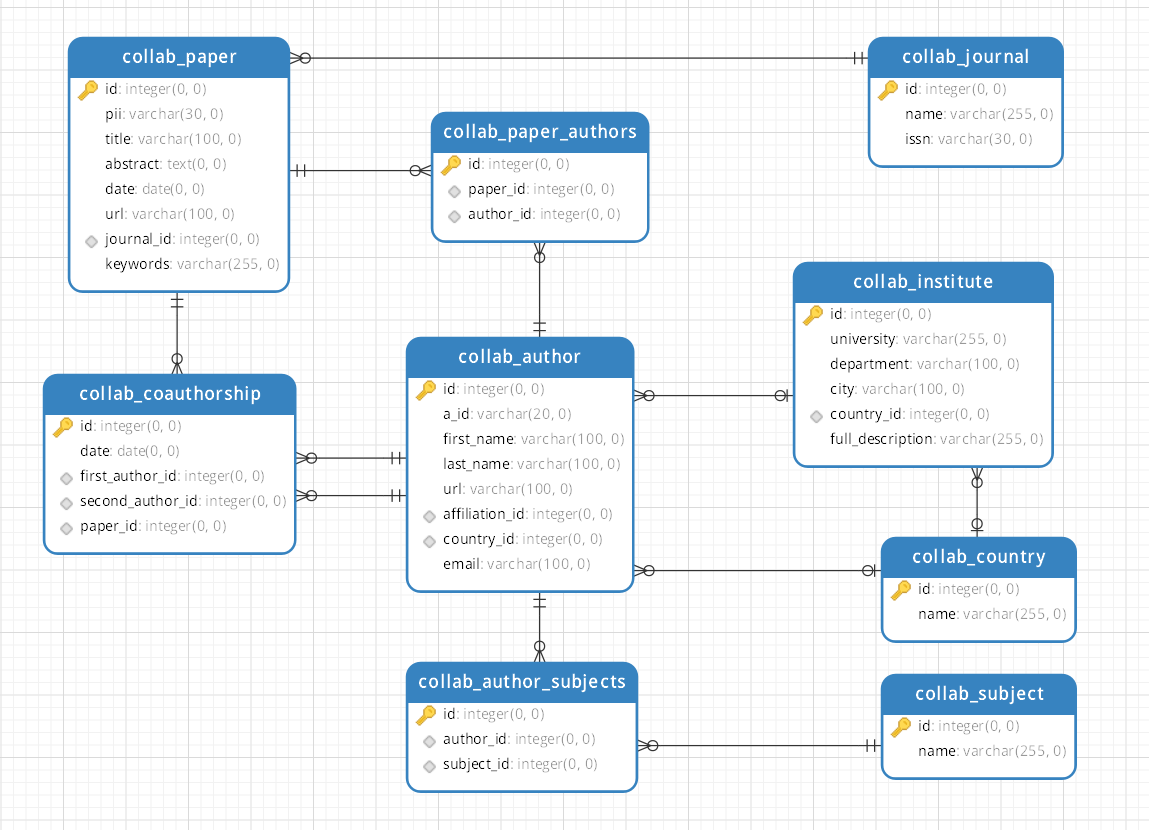
\includegraphics[width=\textwidth]{image/database.png} 
\caption{Cơ sở dữ liệu}
\end{figure}

% first way:
\begin{description}
    \item[collab\_author:] thông tin về tác giả (id, a\_id, first\_name, last\_name, url, affiliation\_id, country\_id, email)
    \item[collab\_coauthorship:] thông tin đồng tác giả (id\_date, first\_author\_id, second\_author\_id, paper\_id) 
    \item[collab\_paper:] thông tin bài báo (id, pii, title, abstract, date, url, journal\_id, keywords)
    \item[collab\_subject:] thông tin lĩnh vực (id, name)
    \item[collab\_author\_subject:] thông tin tác giả nghiên cứu lĩnh vực nào (id, author\_id, subject\_id)
    \item[collab\_paper\_authors:] bảng thông tin về những tác giả viết chung một bài báo (id, paper\_id, author\_id)
\end{description}

\subsection{Truy vấn cơ sở dữ liệu}

\indent Truy vấn thông tin bài báo và hai tác giả cùng viết bài báo đó

\begin{lstlisting}[language=SQL, caption=Đồng tác giả]

create table co_author as
select pa1.paper_id,
			pa1.author_id as id_author_1,
			pa2.author_id as id_author_2
from collab_paper_authors pa1
join collab_paper_authors pa2
on pa1.paper_id = pa2.paper_id
and pa1.author_id < pa2.author_id
order by pa1.paper_id

\end{lstlisting}

\indent Truy vấn tạo nên bảng ứng viên gồm thông tin (ID) của hai tác giả

Cho mạng đồng tác giả $G^T=(V^T, E^T, P^T, T1)$ thì (u, v) là một cặp ứng viên nếu:
$\exists p \in P^{T1}, t \in T1: (u, v, p, t) \in E^{T1}$ hoặc $\exists z \in V^{T1}, (p_1, p_2) \in P^{T1}, (t_1, t_2) \in T1: (u, z, p_1, t_1), (u, v, p_2, t_2) \in E^{T1}$

\begin{lstlisting}[language=SQL, caption=Ứng viên đồng tác giả]

create table potential_co_author as (

	select co1.id_author_2 as id_author_1,
				co2.id_author_2 as id_author_2,
	from co_author co1
	join co_author co2
	on co1.id_author_1 = co2.id_author_1
	and co1.id_author_2 < co2.id_author_2
	
	union
	
	select co2.id_author_1 as id_author_1,
				co1.id_author_2 as id_author_2
	from co_author co1
	join co_author co2
	on co1.id_author_1 = co2.id_author_2
	and co1.id_author_2 > co2.id_author_1
	
	union
	
	select co1.id_author_1 as id_author_1,
				co2.id_author_1 as id_author_2
	from co_author co1
	join co_author co2
	on co1.id_author_2 = co2.id_author_2
	and co1.id_author_1 < co2.id_author_1
	
	union
	
	select co.id_author_1 as id_author_1,
				co.id_author_2 as id_author_2
	from co_author co
)

\end{lstlisting}

\subsection{Các kịch bản truy vấn khác}

\subsubsection{Truy vấn giới hạn số lượng}

\indent Truy vấn giới hạn số lượng các bản ghi để tiện cho việc tính toán nhanh và kiểm thử với số lượng khác nhau:

\begin{lstlisting}[language=SQL, caption=Truy vấn giới hạn số lượng]

	create_paper_table = ("create table paper_" + num_records + 
                            " as select p.id, p.date from collab_paper p \
                            limit " + num_records
                            )

	create_paper_authors_table = ("create table paper_authors_" + num_records + 
                            " as select pa.* from collab_paper_authors pa \
                            where pa.paper_id in (select id from paper_" + num_records + ")"
                            )

	create_author_table = ("create table author_" + num_records + 
                            " as select a.id, a.affiliation_id, ins.university, a.country_id from collab_author a \
                            left join collab_institute ins \
                            on a.affiliation_id = ins.id  \
                            where a.id in (select distinct pa.author_id from paper_authors_" + num_records + " pa)"
                            )       

	create_co_authors_table = ("create table co_author_" + num_records +
                                    " as select pa1.paper_id, pa1.author_id as id_author_1, pa2.author_id as id_author_2 \
                                    from paper_authors_" + num_records + " pa1 \
                                    join paper_authors_" + num_records + " pa2 \
                                    on pa1.paper_id = pa2.paper_id and pa1.author_id < pa2.author_id order by pa1.paper_id"
                                )       


\end{lstlisting}

\subsubsection{Truy vấn theo lát cắt thời gian: điểm cắt}

\indent Dựa theo kịch bản động, lấy điểm cắt thời gian chia ra hai khoảng thời gian T1 và T2:

\begin{lstlisting}[language=SQL, caption=Truy vấn theo lát cắt thời gian: điểm cắt]

	sliced_query = ("create table " + name + " as \
                           select co.paper_id, co.id_author_1, co.id_author_2 from co_author_" + num_records + " co \
                           join paper_" + num_records + " p \
                           on co.paper_id = p.id \
                           where p.date < '" + time_slice + "'")


\end{lstlisting}

\subsubsection{Truy vấn theo khoảng thời gian}

\indent Truy vấn các bản ghi giới hạn khoảng thời gian nằm giữa hai mốc thời điểm

\begin{lstlisting}[language=SQL, caption=Truy vấn theo lát cắt thời gian: khoảng cắt]

	create_paper_table = ("create table sub_db.paper" +  
                            " as select p.id, p.date from collab_paper p \
                            where p.journal_id in (" + ','.join(topics) + ") \
                            and substr(p.date,1,4) >= '" + from_date + "' \
                            and substr(p.date,1,4) <= '" + to_date + "'"
                            )

	create_paper_authors_table = ("create table sub_db.paper_authors" +  
                            " as select pa.* from collab_paper_authors pa \
                            where pa.paper_id in (select id from sub_db.paper)"
                            )

	create_author_table = ("create table sub_db.author" +  
                            " as select a.id, a.affiliation_id, ins.university, a.country_id from collab_author a \
                              left join collab_institute ins \
                              on a.affiliation_id = ins.id  \
                            where a.id in (select distinct pa.author_id from sub_db.paper_authors pa)"
                            )       


\end{lstlisting}

\subsubsection{Truy vấn thời gian của các chủ để}

\indent Thông tin cơ sở dữ liệu gồm bốn chủ đề Biophysical Journal, Journal of Molecular Biology, Chemical Physics Letters, Biochemical and Biophysical Research Communications, truy vấn thời gian xuất hiện của những bài báo nằm trong một hoặc nhiều chủ đề trên. Đồng thời với các truy vấn khác cũng tương tự:

\begin{lstlisting}[language=SQL, caption=Truy vấn thời gian của các chủ đề]

	get_dates_query(topics) = ("select distinct p.date from collab_paper p \
                            where p.journal_id in (" + ','.join(topics) + ")")


\end{lstlisting}

\subsubsection{Truy vấn mức sâu hơn đồng tác giả}

\indent Với hệ ứng viên đồng tác giả (ta gọi là bậc 1) khi truy vấn ứng viên đồng tác giả thêm i lần nữa, ta có hệ ứng viên đồng tác giả với mức sâu $i + 1$ (bậc $i + 1$)

\begin{lstlisting}[language=Python, caption=Truy vấn mức sâu đồng tác giả]

def create_potential_co_authors():
    num_records = request.get_json()["num_records"]
    level = request.get_json()["level"]
    #time_slice = request.get_json()["time_slice"]
    # name_of_sliced_co_author = slice_co_author(num_records, time_slice)

    temp = "co_author_" + num_records

    message = []
    with sqlite3.connect(db_path) as conn:
        cur = conn.cursor()
        for i in range(level):
            if i > 0:
                temp = "potential_co_author_" + num_records + "_" + str(i)
            create_potential_co_authors_table = ("create table potential_co_author_" + num_records + "_" + str(i+1) 
                                            + " as \
                                                select co1.id_author_2 as id_author_1, co2.id_author_2 as id_author_2 \
                                                from " + temp + " co1 \
                                                join " + temp + " co2 \
                                                on co1.id_author_1 = co2.id_author_1 \
                                                and co1.id_author_2 < co2.id_author_2 \
                                                union \
                                                select co2.id_author_1 as id_author_1, co1.id_author_2 as id_author_2 \
                                                from " + temp + " co1 \
                                                join " + temp + " co2 \
                                                on co1.id_author_1 = co2.id_author_2 \
                                                and co1.id_author_2 > co2.id_author_1 \
                                                union \
                                                select co1.id_author_1 as id_author_1, co2.id_author_1 as id_author_2 \
                                                from " + temp + " co1 \
                                                join " + temp + " co2 \
                                                on co1.id_author_2 = co2.id_author_2 \
                                                and co1.id_author_1 < co2.id_author_1 \
                                                union \
                                                select co.id_author_1, co.id_author_2 \
                                                from " + temp + " co")
            name = "potential_co_author_" + num_records + "_" + str(i+1)
            cur.execute(check)


\end{lstlisting}


\section{Tính toán các độ đo liên kết}

\indent Mức độ liên kết của một cặp tác giả trong một mạng đồng tác giả thường được lượng hóa bởi các độ đo liên kêt được trích xuât từ các tập $E^T, A^T$. Dưới đây là một số độ đo thông dụng. Các độ đo liên kết này có thể áp dụng trong nhiều loại mạng xã hội khác nhau, không chỉ riêng cho mạng đồng tác giả. \\

\indent Để tính các độ đo này dễ dàng, đồ thị đồng tác giả được tạo ra và biểu diễn dưới dạng danh sách kề (adj). Trọng số của mỗi cạnh trong đồ thị được tính bằng số bài báo viết chung giữa 2 tác giả. \\

\noindent Chú ý: hiện các độ đo đang được cài đặt dưới hai dạng có trọng số (weighted) và không trọng số (unwieghted).

\subsubsection{Tính toán trọng số cạnh của đồ thị đồng tác giả: Link Value}

\indent Trọng số cạnh của đồ thị đồng tác giả là tổng số lượng các bài báo chung của hai tác giả, Link Value:  $w_{ij}$

\begin{lstlisting}[language=Python, caption=Trọng số của đồ thị đồng tác giả]

def list_co_authors_before_t(u, t, adj):
    res = []
    for v in adj[u].keys():
        for year in adj[u][v].years:
            if year <= t:
                res.append(v)
                break
    return res

def get_weight_before_t(u,v,adj,t):
    old_w = adj[u][v].w
    cnt = 0
    for year in adj[u][v].years:
        if year > t: 
            cnt += 1
    return old_w - cnt

\end{lstlisting}

\subsection{Độ đo dựa trên lân cận: Neighbour-based metrics}

\subsubsection{Độ đo Common Neighbours}

Độ đo Common Neighbours giữa hai nút u và v được tính bằng số lượng nút lân cận chung của u và v. Số lượng nút lân cận chung càng cao thì độ tương đồng Common Neighbours càng lớn, do đó khả năng (u), (v) có liên kết trong tương lai càng cao. 

\begin{center}
 CommonNeighbours(u, v) =  $|T(u) \cap T(v)|$
\end{center}


\begin{lstlisting}[language=Python, caption=Độ đo Common Neighbours]

def CommonNeighbor(id1, id2, adj, t):
    co_id1 = list_co_authors_before_t(id1, t, adj)
    co_id2 = list_co_authors_before_t(id2, t, adj)
    common_neighbors = list(set(co_id1) & set(co_id2))
    # unweighted
    unweighted_res = len(set(co_id1) & set(co_id2))
    # weighted
    weighted_res = 0
    for z in common_neighbors:
        w_id1_z = get_weight_before_t(id1, z, adj, t)
        w_id2_z = get_weight_before_t(id2, z, adj, t)
        weighted_res += (w_id1_z + w_id2_z) / 2
    return {'unweighted' : unweighted_res, 'weighted' : weighted_res}


\end{lstlisting}

\subsubsection{Độ đo Adamic - Adar}

Độ đo Adamic - Adar quan sát thêm số lượng nút lân cận của từng lân cận chung. Với z là lân cận chung của cả u và v thì độ đo Adamic / Adar tỉ lệ  nghịch với số lượng nút lân cận của z tính theo logarithm. 

\begin{center}
AdamicAdar(u, v) = $\Sigma_{z \in T(u) \cap T(v)} . \frac{1}{log(|T(z)|)}$
\end{center}

\begin{lstlisting}[language=Python, caption=Độ đo Adamic - Adar]

def AdamicAdar(id1, id2, adj, t):
    # {z}
    co_id1 = list_co_authors_before_t(id1, t, adj)
    co_id2 = list_co_authors_before_t(id2, t, adj)
    common_neighbors = list(set(co_id1) & set(co_id2))
    # unweighted
    unweighted_res = 0
    for z in common_neighbors:
        co_z = list_co_authors_before_t(z, t, adj)
        unweighted_res += 1 / (math.log(len(co_z)))
    # weighted
    weighted_res = 0
    for z in common_neighbors:
        w_id1_z = get_weight_before_t(id1, z, adj, t)
        w_id2_z = get_weight_before_t(id2, z, adj, t)
        numerator = (w_id1_z + w_id2_z) / 2
        denominator = 0
        co_z = list_co_authors_before_t(z, t, adj)
        for i in co_z:
            w_z_i = get_weight_before_t(z, i, adj, t)
            denominator += w_z_i
        denominator = math.log(denominator)
        weighted_res += numerator / denominator
    return {'unweighted' : unweighted_res, 'weighted' : weighted_res}

\end{lstlisting}


\subsubsection{Độ đo Jaccard's Coeficient}

Độ đo Jaccard's Coefficient giữa hai nút u và v được tính bằng tỉ lệ số lượng lân cận chung trên tổng số lân cận của hai nút.

\begin{center}
JaccardsCoefficient(u, v) = $\frac{T(u) \cap T(v)}{T(u) \cup T(v)}$
\end{center}

\begin{lstlisting}[language=Python, caption=Độ đo Jaccard's Coefficient]

def JaccardCoefficient(id1, id2, adj, t):
    co_id1 = list_co_authors_before_t(id1, t, adj)
    co_id2 = list_co_authors_before_t(id2, t, adj)
    # unweighted
    unweighted_res = len(set(co_id1) & set(co_id2)) / len(set(co_id1).union(set(co_id2)))
    # weighted
    weighted_res = unweighted_res
    return {'unweighted' : unweighted_res, 'weighted' : weighted_res}

\end{lstlisting}


\subsubsection{Độ đo Preferential Attachment}

Độ đo Preferential Attachment thể hiện hai nút càng có nhiều lân cận (bậc càng lớn) thì càng có cơ hội liên kết với nhau trong tương lai.

\begin{center}
PreferentialAttachment(u, v) = |T(u) x T(v)|
\end{center}

\begin{lstlisting}[language=Python, caption=Độ đo Preferential Attachment]

def PreferentialAttachment(id1, id2, adj, t):
    co_id1 = list_co_authors_before_t(id1, t, adj)
    co_id2 = list_co_authors_before_t(id2, t, adj)
    # unweighted
    unweighted_res = len(co_id1) * len(co_id2)
    # weighted
    id1_contri = 0
    for z in co_id1:
        w_id1_z = get_weight_before_t(id1, z, adj, t)
        id1_contri += w_id1_z
    id1_contri /= len(co_id1)

    id2_contri = 0
    for z in co_id2:
        w_id2_z = get_weight_before_t(id2, z, adj, t)
        id2_contri += w_id2_z
    id2_contri /= len(co_id2)
    weighted_res = id1_contri * id2_contri
    return {'unweighted' : unweighted_res, 'weighted' : weighted_res}

\end{lstlisting}

\subsubsection{Độ đo Resource Allocation}

Độ đo Resource Allocation có công thức tương tự như Adamic Adar, chỉ có khác biệt ở phần mẫu số là số lượng lân cận của z.

\begin{center}
ResourceAllocation(u, v) = $\Sigma_{z \in T(u) \cap T(v)} . \frac{1}{|T(z)|}$
\end{center}

\begin{lstlisting}[language=Python, caption=Độ đo Resource Allocation]

def ResourceAllocation(id1, id2, adj, t):
    # {z}
    co_id1 = list_co_authors_before_t(id1, t, adj)
    co_id2 = list_co_authors_before_t(id2, t, adj)
    common_neighbors = list(set(co_id1) & set(co_id2))
    # unweighted
    unweighted_res = 0
    for z in common_neighbors:
        co_z = list_co_authors_before_t(z, t, adj)
        unweighted_res += 1 / (len(co_z))
    # weighted
    weighted_res = 0
    for z in common_neighbors:
        w_id1_z = get_weight_before_t(id1, z, adj, t)
        w_id2_z = get_weight_before_t(id2, z, adj, t)
        numerator = (w_id1_z + w_id2_z) / 2
        co_z = list_co_authors_before_t(z, t, adj)
        denominator = 0
        for i in co_z:
            w_z_i = get_weight_before_t(z, i, adj, t)
            denominator += w_z_i
        weighted_res += numerator / denominator
    return {'unweighted' : unweighted_res, 'weighted' : weighted_res}


\end{lstlisting}


\subsection{Độ đo dựa trên đường đi: Path-based metrics}

\subsubsection{Độ đo Shortest Path}

Độ đo Shortest Path được tính bằng nghịch đảo của khoảng cách ngắn nhất giữa hai nút. Trong trường hợp giữa hai nút không có đường đi thì độ đo có giá trị bằng 0.

\begin{center}
ShortestPath(u, v) = $\frac{1}{d(u, v)}$
\end{center}

\begin{lstlisting}[language=Python, caption=Độ đo Shortest Path]
def bfs(s, e, adj, t):     #bfs to find shortest path between s and e
    num_ver = len(adj)
    max_num_edges = num_ver * (num_ver-1) / 2
    if s == e: return 0
    visited = dict.fromkeys(adj.keys(), False)
    dist = dict.fromkeys(adj.keys(), max_num_edges)
    q = []
    q.append(s)
    visited[s] = True
    dist[s] = 0
    while q:
        u = q.pop(0)
        co_u = list_co_authors_before_t(u, t, adj)
        if u == e: return dist[u]
        else:
            for v in co_u:
                if visited[v] == False:
                    q.append(v)
                    visited[v] = True  
                    dist[v] = dist[u] + 1
    return 0

def ShortestPath(id1, id2, adj,t):    # not take w into account
    dist = bfs(id1, id2, adj, t)
    if dist == 0: return 0
    else:   
        return 1 / dist

\end{lstlisting}

\subsubsection{Độ đo Katz Beta}

Độ đo Katz được tính dựa trên việc thống kê tất cả các đường đi giữa hai nút u và v theo độ dài tăng dần. Các đường đi càng dài thì ảnh hưởng tới độ đo càng giảm do chịu tác động của hàm mũ.

\begin{center}
Katz(u, v) = $\sum_{l=1}^{\infty} \beta^l |path_{u, v}^l| = \beta A + \beta A^2 + \beta A^3 $ + ...
\end{center}

trong đó, $path_{u, v}^l$ là tập các đường đi độ dài l từ u đến v; $\beta$ là hằng số tùy chọn. Khi $\beta$ tiến tới 0 thì độ đo trở nên tương tự với độ đo lân cận chung do các đường đi có độ dài lớn đóng gớp rất ít vào kết quả cuối cùng.

\subsubsection{Độ đo Weighted Katz Beta}

Tính toán giống như độ đo Katz Beta nhưng thay $path_{ij}^1 = w_{ij}$

\subsection{Độ đo dựa theo quốc gia và lĩnh vực chuyên môn}

Để so sánh sự tương đồng hay gần gũi giữa hai tác giả, ngoài việc sử dụng các đặc trưng liên kết của mạng, chúng ta còn có thể khai thác thông tin ngữ nghĩa của từng cá nhân tác giả. Một tác giả hay một nhà nghiên cứu được đặc trưng bởi một số thông tin như quốc tịch, nơi làm việc và lĩnh vực chuyên môn mà họ nghiên cứu. Các tác giả có chung những đặc điểm trên cũng thường có khả năng liên kết trong tương lai cao hơn bình thường.

\subsubsection{Độ đo Common Country}

Xét tập tác giả V = {$v_1, v_2, ..., v_N$}, trong đó tác giả $v_i$ được đặc trưng bởi hai thuộc tính là quốc tịch và nơi công tác ký hiệu bằng $affil_country(v_i)$ và $affil_university(v_i)$. Ta có hàm so sánh sự giống nhau về nơi công tác và quốc tịch giữa hai hoặc nhiều tác giả:

\begin{center}

\[
  sim\_work (v_1, v_2, ..., v_n) =
  \begin{cases}
    2 \text{ if} & affil_{university}(v_1) = affil_{university}(v_2) = ... = affil_{university}(v_n) \\
    1 \text{ if} & affil_{country}(v_1) = affil_{country}(v_2) = ... = affil_{country}(v_n) \\
    0 \text{ if} & otherwise
  \end{cases}
\]

\end{center}

Độ đo tương đồng giữa hai tác giả u và v theo cộng đồng quốc gia được tính theo công thức:

\begin{center}

CommonCountry(u, v) = $sim\_work(u, v)$ + $\Sigma_{z \in T(u) \cap T(v)} . sim\_work(z, u, v)$

\end{center}

\begin{lstlisting}[language=Python, caption=Độ đo Common Country]

def CommonCountry(adj, list_vertices, records, num_records, max_time, label_type, time_slice):  # records of potential_co_author
    # return list of scores of each pair
    CommonCountry_list = []
    
    # query country_id and affiliation_id of 2 authors
        
    def sim_work_2(id1, id2):
        if list_vertices[id1].university == list_vertices[id2].university: return 2
        elif list_vertices[id1].country_id == list_vertices[id2].country_id: return 1
        else: return  0

    def sim_work_3(id1, id2, id3):
        if list_vertices[id1].university == list_vertices[id2].university and list_vertices[id1].university == list_vertices[id3].university:
            return 2
        elif list_vertices[id1].country_id == list_vertices[id2].country_id and list_vertices[id1].country_id == list_vertices[id3].country_id:
            return 1
        else: return 0
    if label_type == "dynamic":
        for row in records:
            id1 = row[0]
            id2 = row[1]
            if id2 in adj[id1].keys(): 
                t = max(adj[id1][id2].years)
                comm_country_score = sim_work_2(id1, id2)    
                co_id1 = list_co_authors_before_t(id1, t, adj)
                co_id2 = list_co_authors_before_t(id2, t, adj)
                common_neighbors = list(set(co_id1) & set(co_id2))
                for z in common_neighbors:
                    comm_country_score += sim_work_3(id1, id2, z)
                CommonCountry_list.append(comm_country_score)
            else:
                comm_country_score = sim_work_2(id1, id2)    
                co_id1 = list_co_authors_before_t(id1, max_time, adj)
                co_id2 = list_co_authors_before_t(id2, max_time, adj)
                common_neighbors = list(set(co_id1) & set(co_id2))
                for z in common_neighbors:
                    comm_country_score += sim_work_3(id1, id2, z)
                CommonCountry_list.append(comm_country_score)
    if label_type == "static":
        for row in records:
            id1 = row[0]
            id2 = row[1]
            comm_country_score = sim_work_2(id1, id2)    
            co_id1 = list_co_authors_before_t(id1, time_slice, adj)
            co_id2 = list_co_authors_before_t(id2, time_slice, adj)
            common_neighbors = list(set(co_id1) & set(co_id2))
            for z in common_neighbors:
                comm_country_score += sim_work_3(id1, id2, z)
            CommonCountry_list.append(comm_country_score)
            
    return CommonCountry_list

\end{lstlisting}

\subsubsection{Độ đo Common Topic}

Mỗi tác giả trong mạng lưới học thuật còn được đặc trưng bởi các lĩnh vực chuyên môn mà họ quan tâm. Để tìm ra các lĩnh vực chuyên môn này của một tác giả, chúng ta có thể lấy thông tin từ nội dung các bài báo được công bố tron quá khứ của họ. Mô hình chủ để là một trong những phương pháp có thể áp dụng để phân tích các chủ đề từ một tập các bài báo đầu vào. Kết quả của mô hình chủ đề cho ta biết xác suất bài báo p sẽ thiên về chủ đề nào nằm trong số lượng k chủ đề cho trước thể hiện qua vector đặc trưng chủ đề T = $(t_1, t_2, ..., t_k)$. Từ kết quả phân tích chủ đề các bài báo, ta có thể xác định danh sách các chủ đề mà một tác giả có khả năng quan tâm: 
$T_{v_i} = \sum_{j=1}^N T_{ịj} = (t_{i_1}, t_{i_2}, ..., t_{i_k})$ \\\\

Danh sách các lĩnh vực được tác giả quan tâm nhất:
\[
Topics(v_i) = \{j | j \in [1..k] \land t_{ij} > \theta \}
\]

Từ thông tin của các cộng đồng này, ta sẽ xây dựng độ đo liên kết giữa hai tác giả (u, v) dựa trên cộng đồng tác giả theo lĩnh vực chuyên môn như sau:
\[
CommonTopic(u, v) = |Topics(u) \cap Topics(v)| + \Sigma_{z \in T(u) \cap T(v)} |Topics(z) \cap Topics(u) \cap Topics(v)|
\]

\newpage

\section{Chương trình truy vấn thông tin đồng tác giả và độ đo liên kết}

Chương trình sử dụng cơ sở dữ liệu SQLite, ngôn ngữ Python để thao tác tính toán, sử dụng framework Flask Python để xây dựng nên giao diện tương tác.

\subsection{Cấu trúc chương trình}

Chương trình được xây dựng gồm các folder và các file Python:

\begin{itemize}
	\item calculate\_scores.py: Ghi thông tin các độ đo tính được ra file CSV
	\item co\_author\_graph.py: Mô hình hóa dữ liệu đồng tác giả thành đồ thị
	\item define\_scores.py: Tính toán độ đo liên kết theo công thức
	\item instance: Chứa cơ sở dữ liệu gốc và các cơ sở dữ liệu sinh ra khi truy vấn
	\item kat\_score.py: Tính toán độ đo theo đường đi Katz Beta
	\item \_\_pychace\_\_: Folder tự sinh ra khi chạy server Flask
	\item query.py: Truy vấn cơ sở dữ liệu
	\item results: Các file CSV chứa độ đo tính toán được lưu lại
	\item static: Chứa các file CSS tạo giao diện đồ họa
	\item template: Chứa các file giao diện dạng web HTML 
\end{itemize}

\begin{figure}[h]
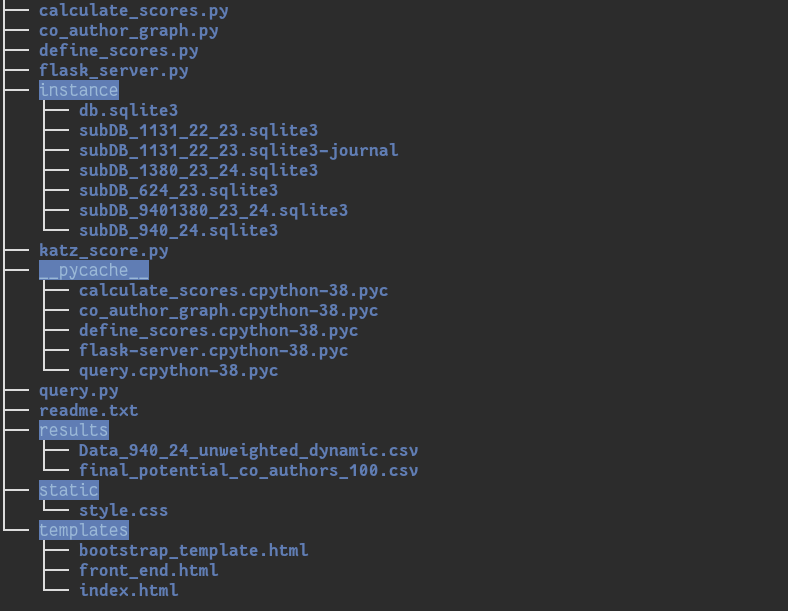
\includegraphics[width=1\textwidth]{image/tree_folder.png}
\caption{Cấu trúc thư mục chương trình}
\end{figure}

\newpage

\subsection{Giao diện chương trình}

\begin{wrapfigure}{r}{0.25\textwidth} %this figure will be at the right
    \centering
    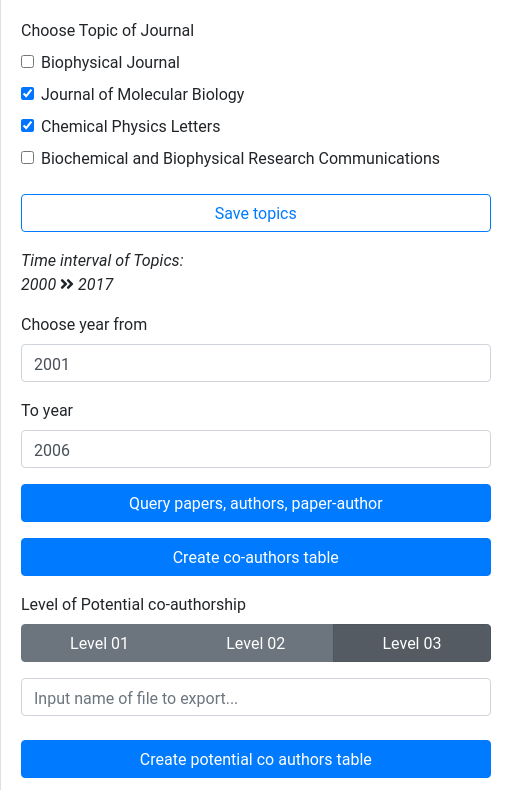
\includegraphics[scale=0.3]{image/overview.png}
\end{wrapfigure}

Dưới đây là thông tin sử dụng của chương trình: \\

Giao diện chương trình gồm tiêu đề Project III, các chủ đề nằm trong cơ sở dữ liệu mẫu: Biophysical Journal, Journal of Molecular Biology, Chemical Physics Letters và Biochemical and Biophysical Research Communications. Nút Save topics sẽ chọn ra những chủ đề và truy vấn ra khoảng thời gian mà các bài báo được viết thuộc các chủ đề đã chọn (2000 đến 2017). Bên dưới là phần chọn khoảng thời gian truy vấn phải đảm bảo nằm trong khoảng thời gian đã hiện bên trên. \\


Chương trình cung cấp hai phím chức năng tiếp theo để truy vấn ra thông tin (số lượng) bài báo, tác giả và hệ tác giả - bài báo được viết. Tiếp đó là mức truy vấn ứng viên đồng tác giả gồm 3 mức là cấp 1, cấp 2 và cấp 3. Trước khi truy vấn ứng viên đồng tác giả, ta có thể đặt tên cho file dữ liệu sẽ được trích xuất ra. \\

%\begin{wrapfigure}{r}{0.25\textwidth} %this figure will be at the right
%    \centering
%    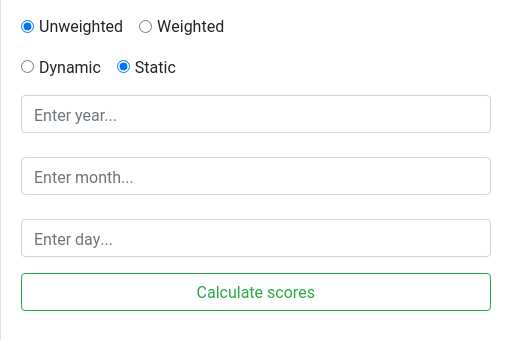
\includegraphics[scale=0.3]{image/static.png}
%\end{wrapfigure}

Sau khi truy vấn ra dữ liệu đồng tác giả, ứng viên đồng tác giả, dữ liệu này sẽ được lưu ra file với tên mặc định hoặc được đặt thủ công (.sqlite3). Tiếp nối điều này, chương trình cho phép ta sử dụng cơ sở dự liệu vừa kết xuất để tính toán độ đo và gán nhãn cho bài toán mạng lưới đồng tác giả. Gồm các chức năng chọn lựa (Unweighted: Không trọng số, Weighted: Có trọng số) và tính toán gán nhãn theo kịch bản (Dynamic: Động, Static: Tĩnh). \\

Thông tin kết quả sẽ được ghi phần cuối của chương trình bao gồm thông tin số lượng các bài báo, tác giả, số lượng danh sách các bài báo - tác giả, đồng tác giả, ứng viên đồng tác giả bậc 1, ứng viên đồng tác giả bậc 2, bậc 3.

\begin{figure}[h]
\begin{subfigure}{.5\textwidth}
  \centering
  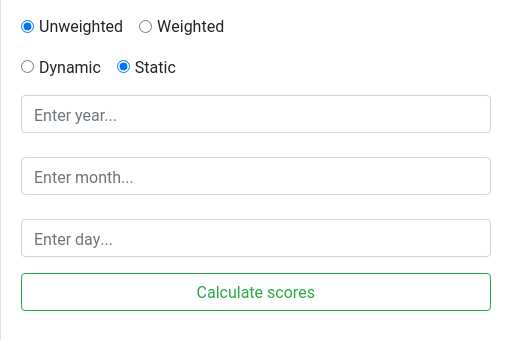
\includegraphics[width=.8\linewidth]{image/static.png}
  \caption{Chọn lựa kịch bản động và tĩnh}
  \label{fig:sfig1}
\end{subfigure}%
\begin{subfigure}{.5\textwidth}
  \centering
  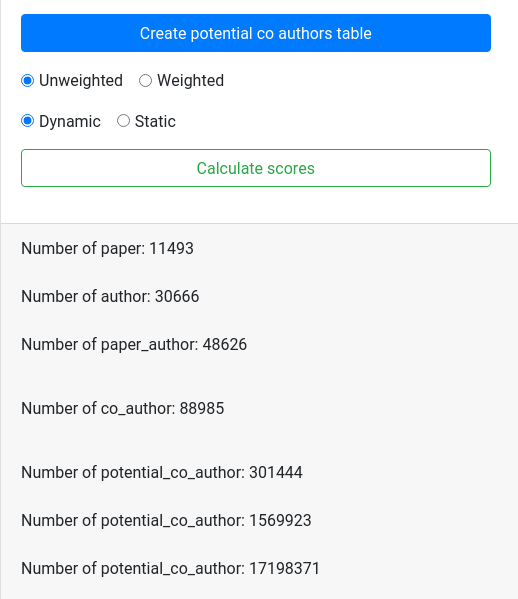
\includegraphics[width=.8\linewidth]{image/query.png}
  \caption{Truy vấn ra các kết quả}
  \label{fig:sfig2}
\end{subfigure}
\caption{Kết quả thử nghiệm chương trình}
\label{fig:fig}
\end{figure}




\newpage

\section{Xây dựng hệ khuyến nghị cộng tác đồng tác giả}


Việc xây dựng hệ khuyến nghị cộng tác bao gồm ba giai đoạn: \\

\indent Thu thập dữ liệu, phân tích, tổ chức dữ liệu: Dữ liệu của hệ thống bao gồm thông tin về các bài báo và tác giả (tiêu đề bài báo, tóm tắt nội dung, từ khóa, thông tin tác giả, ...) từ các tạp chí Chemical Physic Letters, Journal of Molecular Biology và Biochemical and Biophisical Communications của Sciencedirect trong khoảng thời gian 2000-2007 thông qua API của Sciencedirect. \\

\indent Tính toán các độ đo liên kết và tính toán bảng ứng viên \\

\indent Xây dựng mô hình khuyến nghị: Dựa trên mô hình phân lớp Support Vector Machine (SVM) với dữ liệu đã được gán nhãn của bảng ứng viên bao gồm học mô hình từ dữ liệu huấn luyện là bảng ứng viên đã gán nhãn, lưu trữ mô hình và sử dụng mô hình để tính toán khuyến nghị đồng tác giả (huấn luyện, kiểm thử và gợi ý).

\newpage

\section{Danh mục tài liệu tham khảo}

\begin{enumerate}
	\item Miilen Pavlov$^{1, 2}$, Ryutaro Ichise, "Finding Experts by Link Prediction in Co-authorship Networks", 2007
	\item Zervas P, Tsitmidelli A, Sampson DG, Chen NS, Kinshuk (2014), Studying research collaboration pat\-terns via co\-authorship analysis in the field of Tel: The case of educational technology \& society journal, Educ Technol Soc 17(4), pp 1–16
	\item  M. A. Brandão, M. M. Moro, G. R. Lopes, and J. P. M. Oliveira (2013), Using link semantics to recommend collaborations in academic social networks, in Proc.22nd Int. Conf. World Wide Web Companion (WWW Companion), pp.833–840
	\item  W. Glänzel and A. Schubert (2005), Analysing scientific networks through co-authorship, in Handbook of Quantitative Science and Technology Research.New York, NY, USA: Springer-Verlag, pp. 257–276.
	\item Pham Minh Chuan, Le Hoang Son, Mumtaz Ali, Tran Dinh Khang, Le Thanh Huong, Nilanjan Dey (2018), Link Prediction in Co-authorship Networks based on Hybrid Content Similarity Metric, Applied Intelligence, 48(8), ISSN: 0924-669X. Doi: 10.1007 s10489-017-1086-x, pp. 2470–2486
\end{enumerate}


\end{document}